\section{Method and Discussion}
 The pipeline is depicted in \autoref{img:flwPipe}. It consists of a first stage, wherein the raw data is trimmed to remove irrelevant data at the start and end. The same stage automatically splits the data according to the selected training ratio of 70:30. From then on, one part of the data is used as training data to train the actual classifier ensemble depicted in \autoref{img:flwClass} and the other is used as test data to rate the trained models\footnote{Validation data and training/testing data were acquired by different people to support the calculation of reliable validation/generalization figures.}.

\begin{figure}[hbtp]
\centering
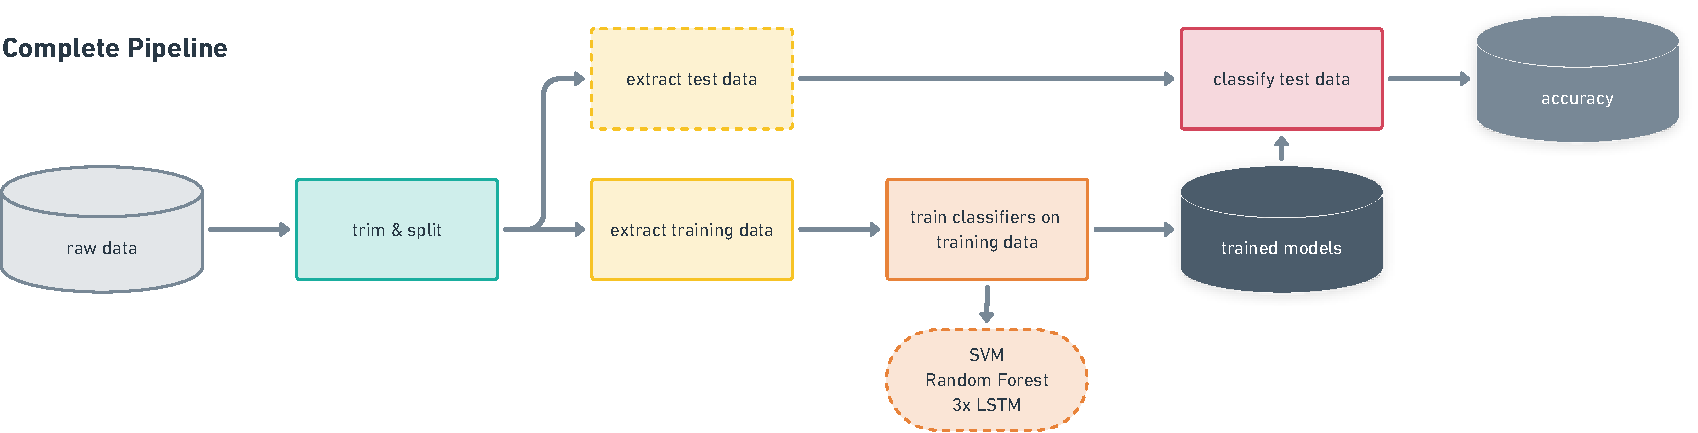
\includegraphics[width=\linewidth]{Flowchart-Pipeline.pdf}
\caption{Flowchart of the complete data processing pipeline}
  \label{img:flwPipe}
\end{figure}

The model itself consists of five classifiers, each with specific settings regarding whether to sort the axes by their mean to compensate for different orientations during data acquisition, which features to use, how many iterations to train and how many hidden units to configure in the \ac{LSTM} layer of the \acp{NN}. \autoref{img:flwClass} shows how the \ac{SVM} and \ac{RF} are feed with features, whereas the \acp{LSTM} are directly working on the time-series data. Depending on the settings, our proposed ensemble operates either in 1-stage or 2-stage stacking scenario. Our test yielded, that the 1-stage stack provides superior testing accuracy, while still working reasonably well on validation data.

\begin{figure}[hbtp]
\centering 
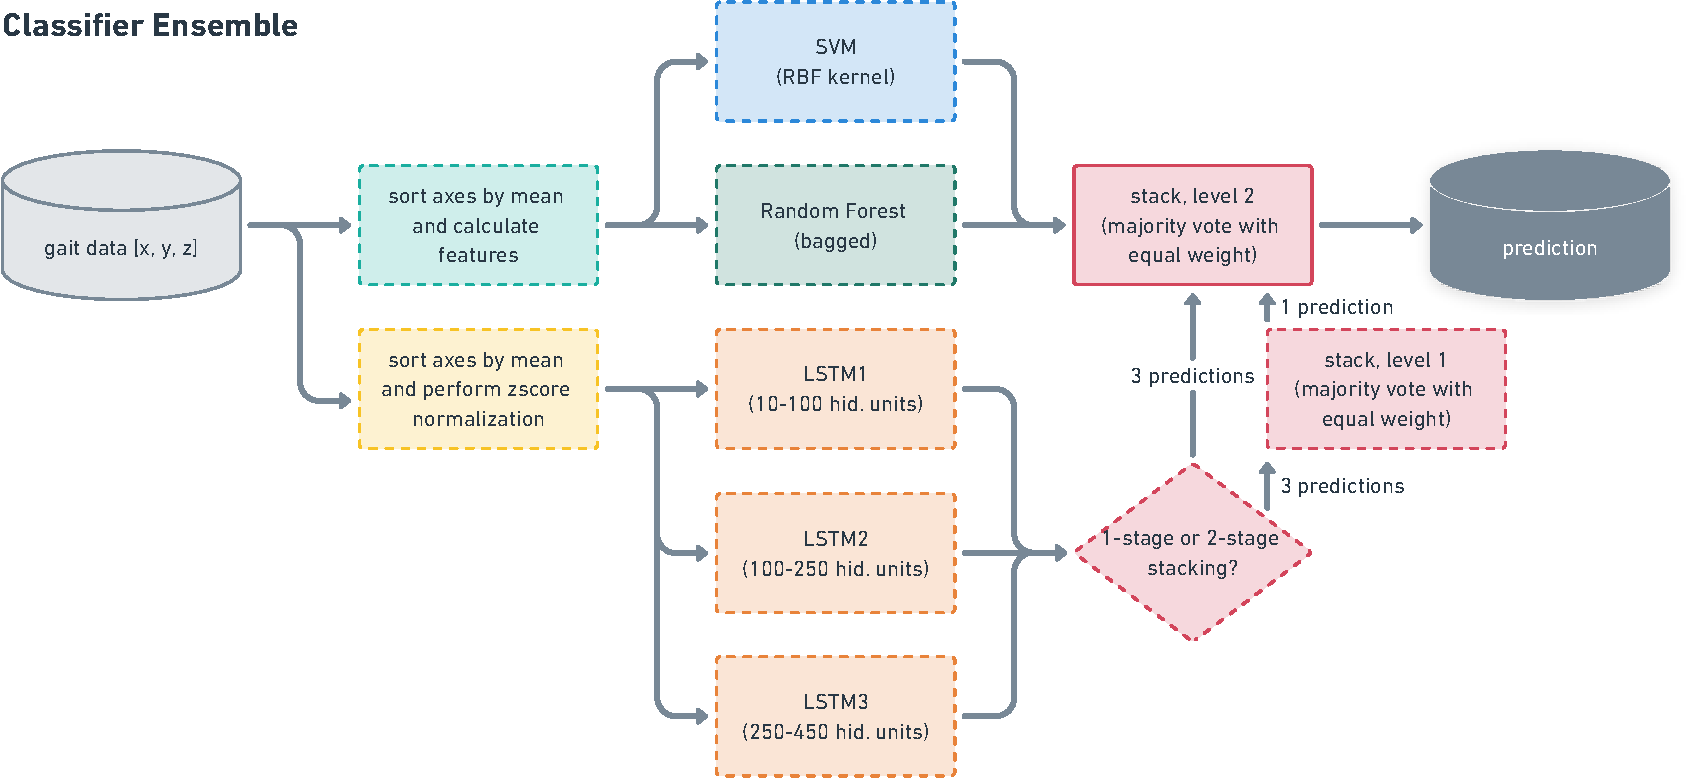
\includegraphics[width=.84\linewidth]{Flowchart-ClassifierEnsemble.pdf}
\caption{Flowchart of classifier ensemble architecture}
  \label{img:flwClass}
\end{figure}

% Optimization Process
The search for the optimal model was done in an iterative manner. The optimization target was chosen as the mean balanced accuracy of the model when applied on training, testing and validation data. In total eleven cycles with an amount of 234 models were trained and evaluated. The results of the 10th cycle are shown in table \ref{tbl:opt_process}. The goal was to determine the impact of nondeterminism introduced by MATLAB's LSTM training procedure by training 20 different models with the final settings. Table \ref{tbl:opt_process} summarizes the results of this cycle and shows a remarkable mean balanced accuracy on test data of almost \unit{99}{\%} for the final settings.
The entry point for this cycle was determined by choosing the most promising model from the previous 9 optimization cycles. There we applied a parameter sweep across all settings.
The final model has a unique combination of outstanding balanced accuracy on test data, good validation performance, fast classification (as \ac{SVM} and \ac{RF} operate with the same feature settings which allows a combined feature extraction), and short training time.
 
%% Tabelle einfügen
\begin{table}[h]
     \centering
     \caption{Statistics on the balanced accuracy of 20 trained models with final settings}
     \begin{tabular}[h]{p{2cm}||p{1cm}|p{1cm}|p{1cm}|p{1cm}}
     Metric & Max [\%]& Min [\%]& Mean [\%]& Std [\%] \\
     \hline
     mean of mean (train, test, val.) &$96.73$&$95.23$&$96.02$&$0.235$\\
     training &$100$&$99.92$&$99.96$&$0.030$\\
     testing &$99.52$&$97.85$&$98.82$&$0.408$\\
     validation &$90.71$&$86.72$&$89.29$&$0.927$  \\
     \end{tabular}
	\\
     \label{tbl:opt_process}
     % Verweis im Text mittels \ref{tbl:beispieltabelle}
   \end{table}

Subsequently, the model with the highest testing accuracy was chosen as it promises to perform well on data acquired by other people with similar movements while still supporting generalization as is indicated by its validation accuracy. The model reached a balanced accuracy on training data of \unit{99.9693}{\%}, on test data of \unit{99.5196}{\%} and on validation data of \unit{90.7076}{\%}.

 % Features + SVM + RF Classifier
The feature-based models \ac{SVM} and \ac{RF} are fed with feature vectors instead of the preprocessed data. Before assessing the features, the axes of acceleration data are sorted by mean value to tackle the problem of varying phone orientation during data recording. Besides basic statistical features like mean and variance, advanced features like the Shannon Entropy or the Wavelet Leader Estimation are evaluated and combined in a feature vector.

While the \ac{SVM} model trains with a maximum number of 200 iterations using randomsearch, the \ac{RF} classifier uses a bagging ensemble technique with 100 iterations.

Further the optimization process yielded the improvement by introducing multiple \ac{LSTM} networks in parallel - each adapting to different time horizons of human gait dynamics. Therefore three networks are placed in parallel with 36, 213 and 378 hidden units respectively. The training was done with a minibatch size of 20 and an epoch limit of 30. Similarly to the feature extraction, an axes-sorting algorithm was implemented and contributed to a higher accuracy.

Figure \ref{img:confmat} depicts the confusion matrix of the final model. The classification procedure runs almost instantaneously while maintaining the mentioned accuracy figures. This supports potential applications in real-time systems like gait classification in phones, smart-watches or similar.

\begin{figure}[hbtp]
\centering 
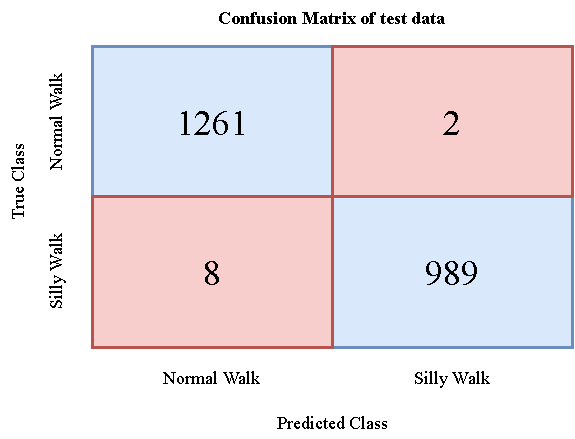
\includegraphics[width=.7\linewidth]{ConfusionMatrix.pdf}
\caption{Confusion Matrix of the final model on the test data}
  \label{img:confmat}
\end{figure}


 
 